\subsection{Control de Versiones, tests unitarios e integración continua}

Desde el inicio del proyecto se ha desarrollado utilizando \emph{GIT} como control de versiones, utilizando la plataforma web \emph{GitHub}, una forja que sirve para alojar proyectos de forma pública y de manera gratuita, aunque se puede crearse una cuenta de pago para tener repositorios privados.

Además, se han realizado tests unitarios utilizando para ello la herramienta \emph{PHPUnit}, lo cual nos permite tener una aplicación sólida y poco propensa a errores, ya que con cada modificación que se realiza se vuelven a pasar los tests para comprobar la estabilidad del código. Otra de las ventajas de realizar tests es que si se encuentra un error, solamente hay que escribir un test para ello y corregirlo, por lo que será imposible que el mismo error se vuelva a repetir en un futuro ya que estará cubierto bajo ese test.

Y por último, por encima de estos dos pilares, se ha realizado integración continua con \emph{Travis CI}, una aplicación web que se sincroniza con la cuenta de \emph{GitHub}, construyendo la aplicación y realizando los tests unitarios cada vez que se realiza un \emph{push} al repositorio.

\begin{figure}[H]
    \centering
    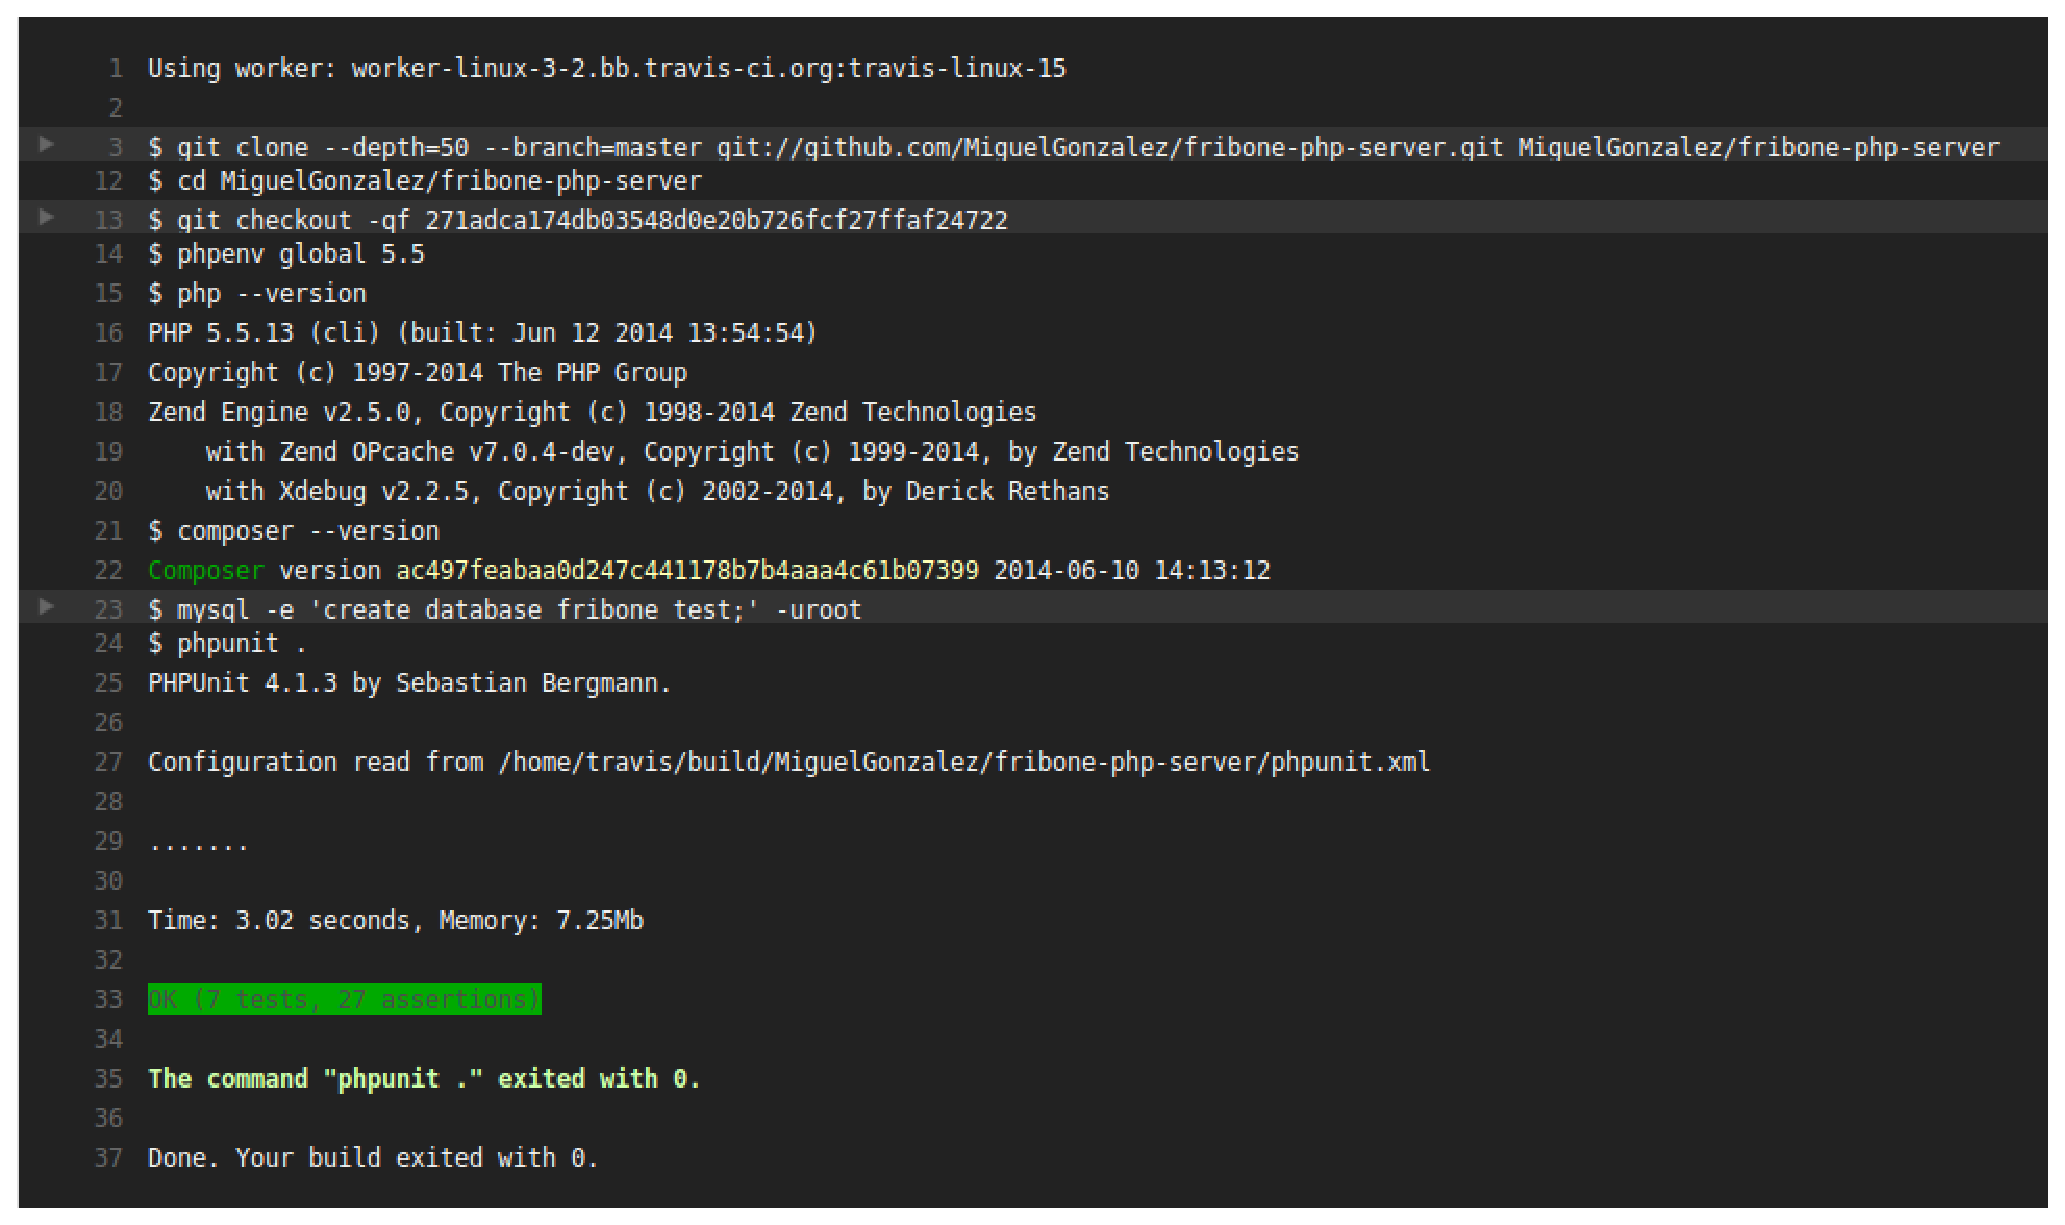
\includegraphics[keepaspectratio,width=0.9\textwidth]{travis-ci-tests.eps}
    \caption{Tets - Travis CI}\label{fig:travis-ci-tests}
\end{figure}